\section{System design}



\subsection{Physical layout}

The more detailed physical layout diagram shows the actual relations of the modules of the system to each other. There are several rapid prototyping technologies working together, all of them based on very high level languages.

The embedded system is running Angström Linux, which is a lightweight linux distribution. It enabled the use of Python and USB Hardware-extensions, a generic cheap USB Bluetooth Dongle and a webcam (The webcam is working, but it’s not supported yet on the software level).
Using Linux as the operating system of the embedded device has the additional advantage of manually controlling and updating the system through SSH.

The HLI and LLI are both implemented in Python. They communicate through function calls implemented via Cython. The actual Controller and Kalman Filter run natively, the .c/.h source code is compiled to .so files by the Cython compiler, which can be imported into the main python software as a static function library.

The source code files are generated by MATLAB Embedded Coder, based on the Simulink model of the control system. The resulting functions are more like objects, containing inner states and member functions, but only one instance can exist of the same controller object.

The GPIOs are controlled from Python as well, using system calls.

\begin{figure}[H]
	\centering
	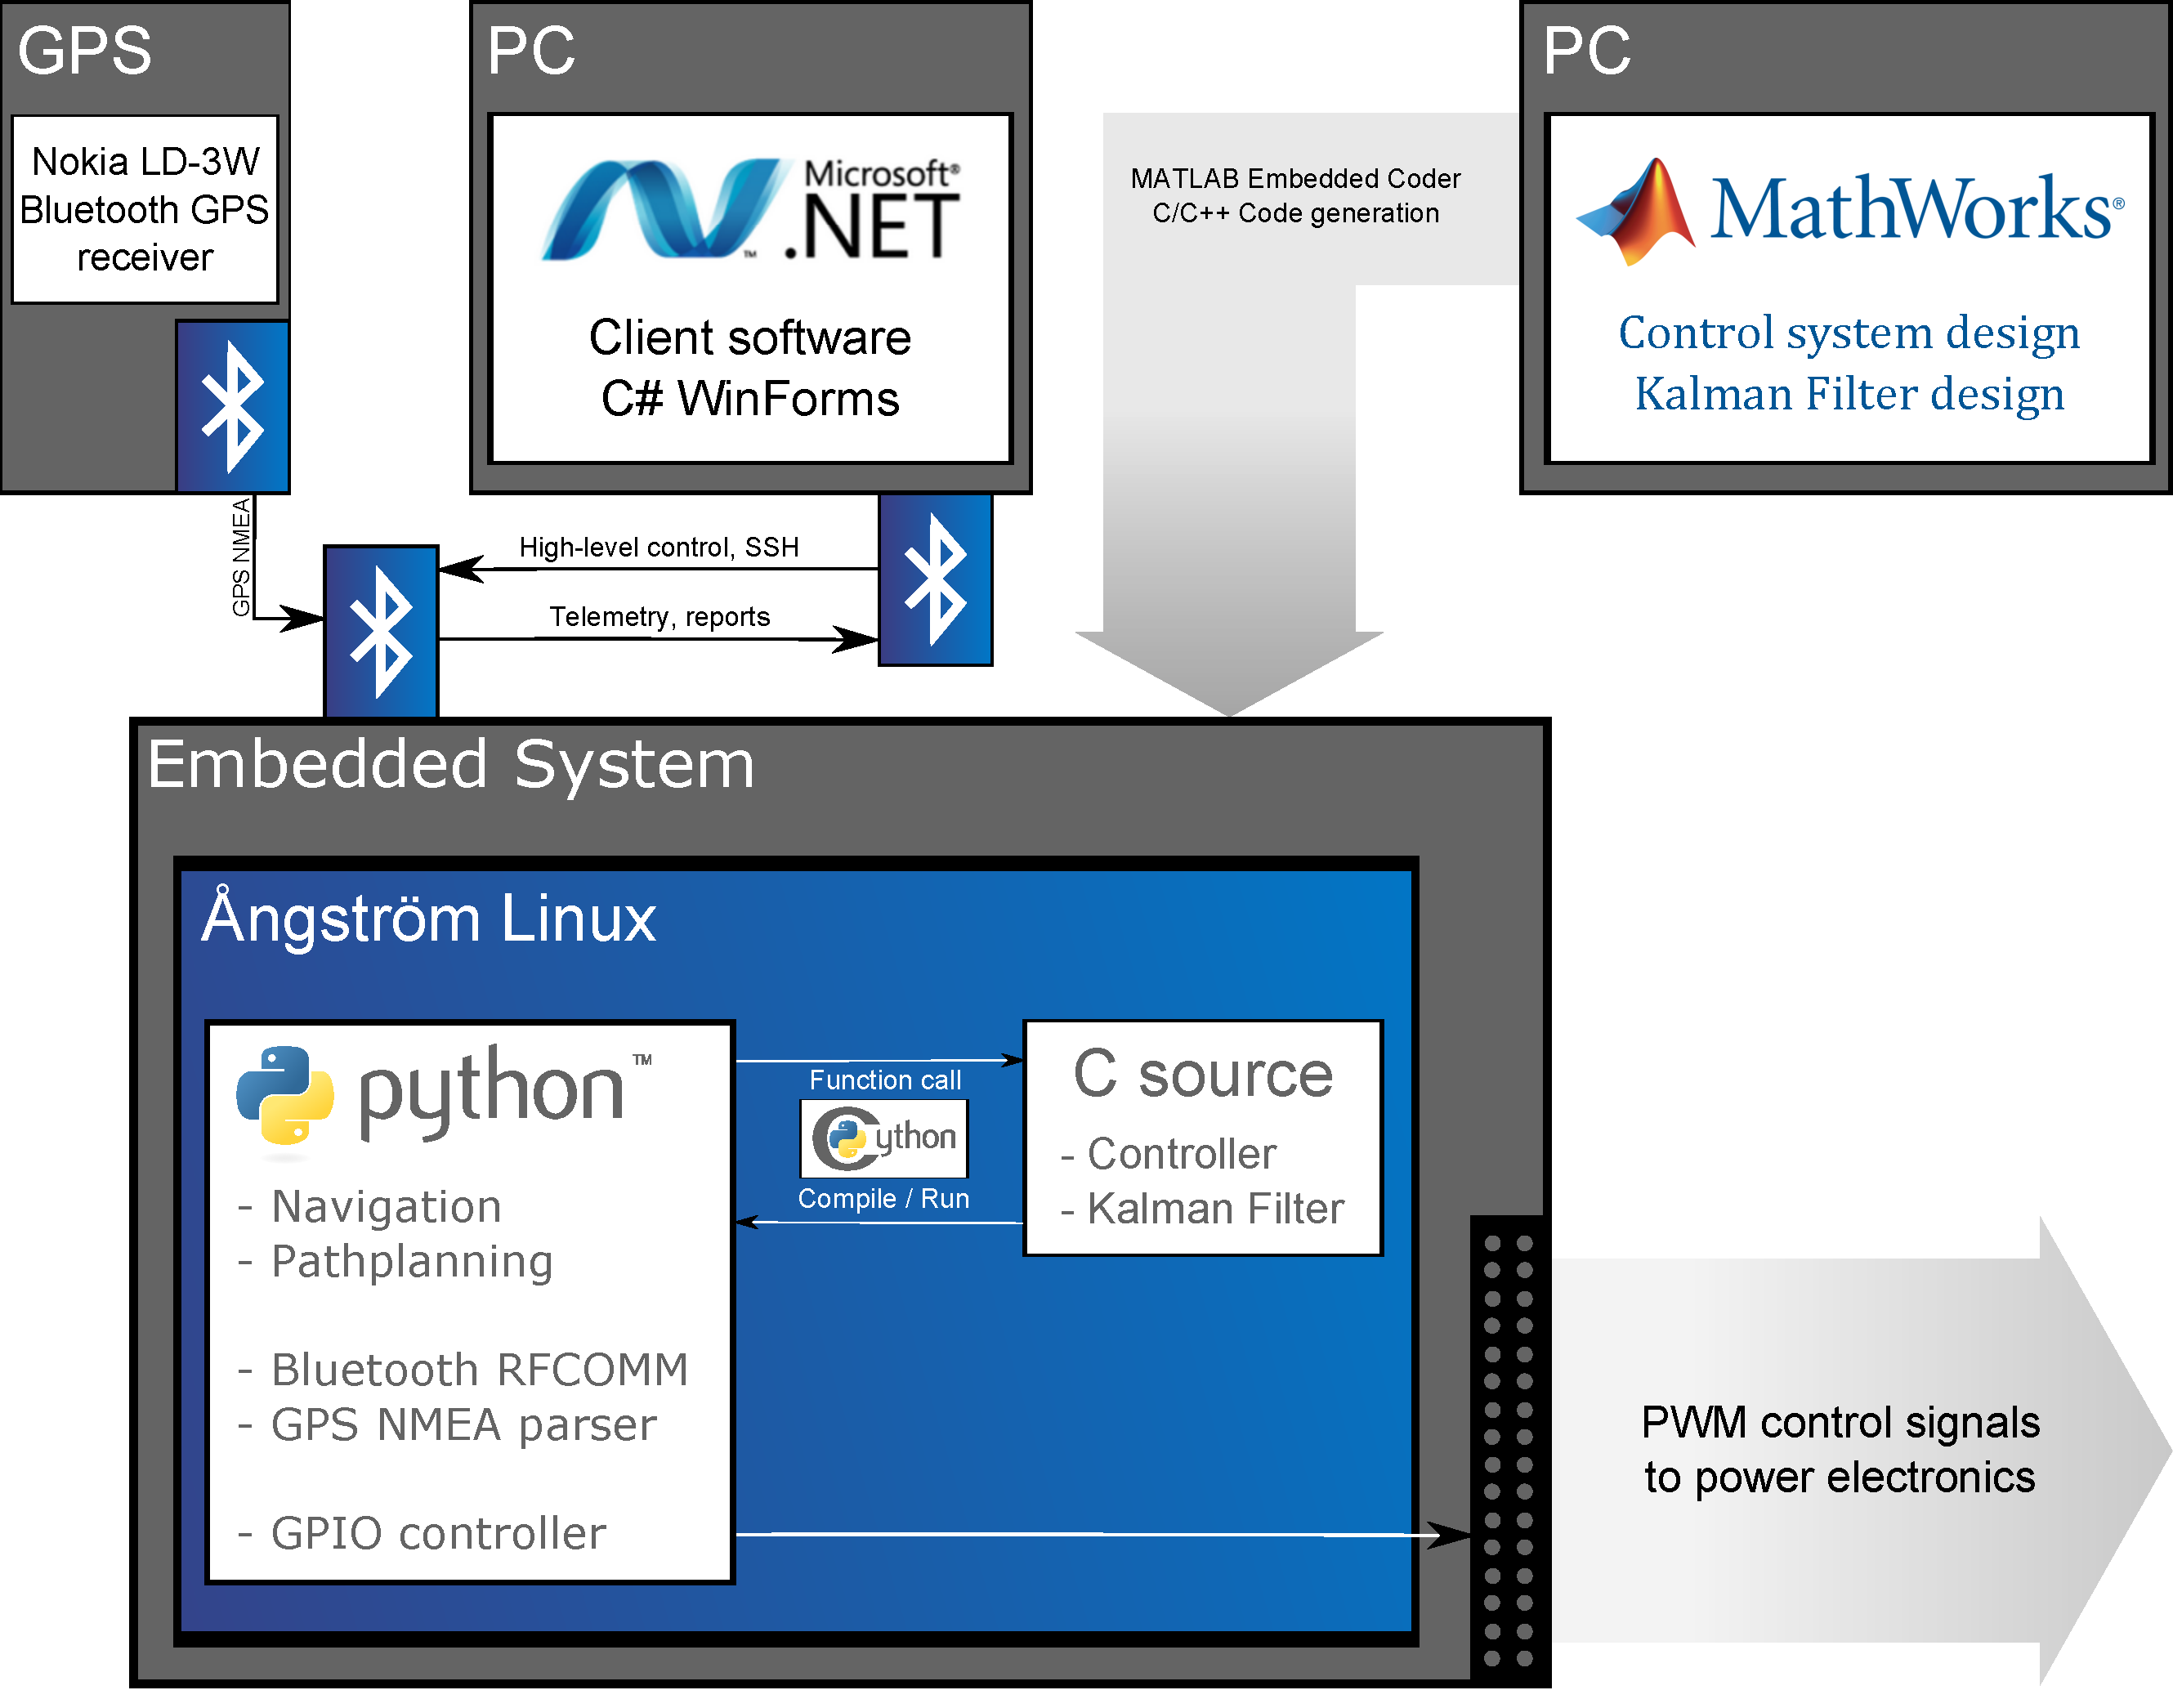
\includegraphics[width=1\textwidth]{img2/PhysicalLayout}
	\caption{The physical layout of the system}
	\label{fig:PhysicalLayout}
\end{figure}

The Embedded system has an USB Bluetooth hardware extension that communicates with the GPS receiver and the Client software.
It’s important to note, that the GPS receiver and the Embedded system are physically close to each other (relative to the scale of the ship), always within the range of the Bluetooth connection. Using wireless communication however enables the distant placement (relative to the scale of the circuit board) in order to ensure high GPS reception and a protected environment for the embedded system as well (e.g.: top of the mast and the belly of the boat).

\subsection{GPS Acquisition}

The localization procedure is implemented by a GPS (Global Positioning System) receiver, connected to the BBB via Bluetooth. The actual device is a Nokia LD-3W GPS device produced for Bluetooth-enabled smartphones without GPS connectivity. The receiver includes a battery with a relatively long life. Solar charging of the device is possible. [wrapfigure]
The Nokia LD-3W transforms the GPS signals to NMEA sentences that can be parsed to extract the current position, speed and much else.

\subsection{Bluetooth connectivity}

\subsection{Sensors and effectors}